A modern \ac{crs} can be deconstructed into several core architectural components, each responsible for a specific aspect of the conversational recommendation process. A conceptual view of how these components interact is shown in Figure~\ref{FIG:CRS_ARCH}. Common building blocks referred to in research are: Interaction Modalities, Underlying Knowledge, and Computational Tasks \cite{SOTA-CRS-SURVEY}.

\begin{figure}[CRS Architectural Components]{FIG:CRS_ARCH}{A conceptual diagram of the core architectural components of a \acl{crs} \cite{CRS-EVALUATION}.}
    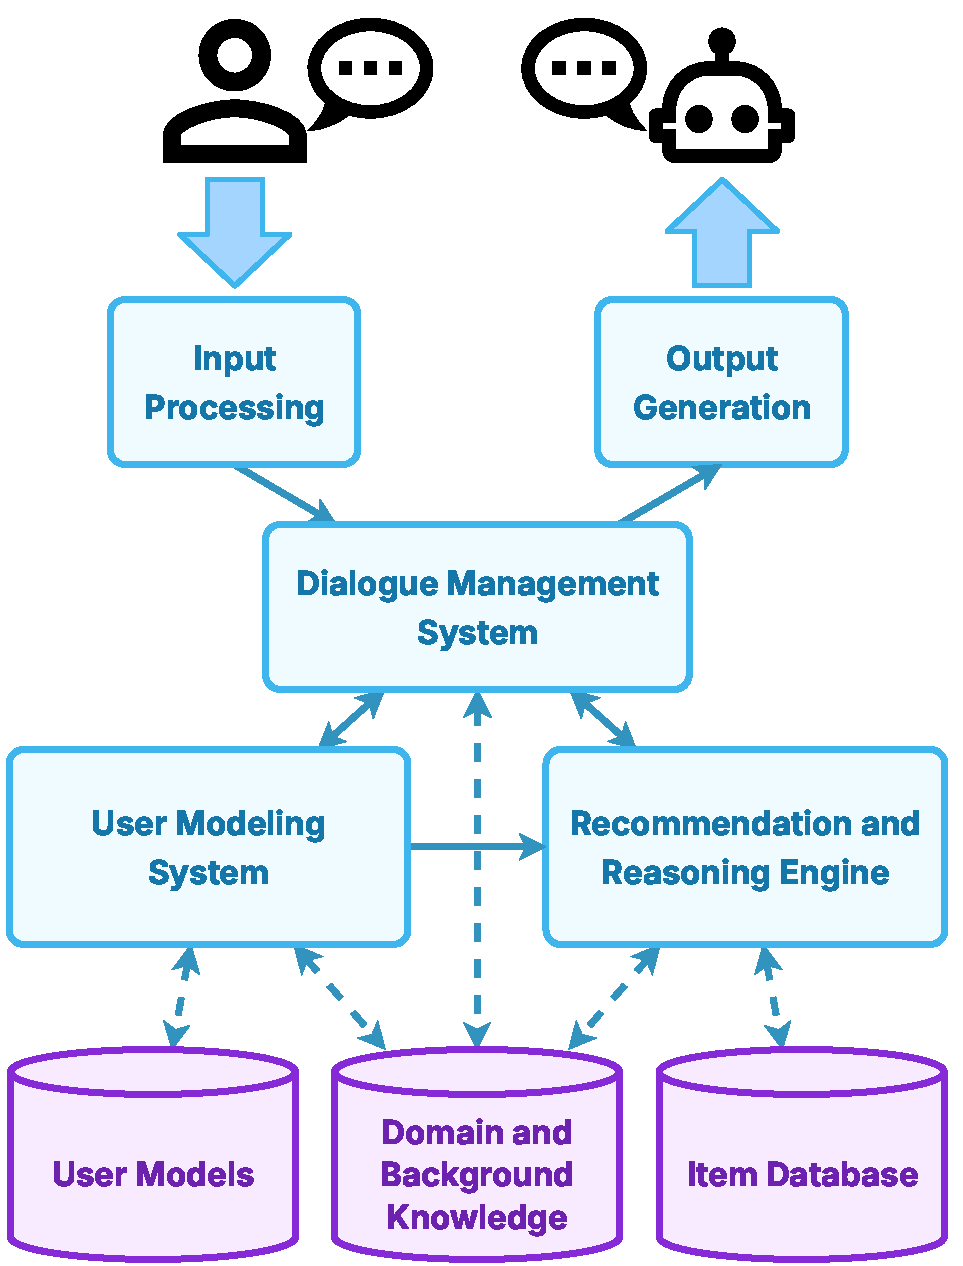
\includegraphics[width=0.6\textwidth]{crs_general_components.pdf}
\end{figure}

\paragraph{Interaction Modalities}
This dimension defines \textit{how} the user and the system interact. It encompasses the \textbf{input/output methods}, which can range from structured inputs like buttons and forms to the more flexible but complex paradigm of natural language text or speech. Many contemporary systems employ a hybrid approach, combining natural language input with visual outputs like interactive item cards \cite{SOTA-CRS-UI}. It also includes the \textbf{interaction initiative}, which determines who leads the dialogue. This can be \textit{system-driven}, where the system asks a series of questions (a model often called ``System Ask, User Respond'' or SAUR); \textit{user-driven}, where the user directs the flow; or \textit{mixed-initiative}, which allows for a more natural back-and-forth and is the most common approach in modern systems \cite[Section 3]{SOTA-CRS-SURVEY}.

\paragraph{Underlying Knowledge and Data}
This category describes the information sources that the \ac{crs} relies upon to function effectively \cite[Section 4]{SOTA-CRS-SURVEY}.
\begin{compactitem}[\textbullet]
    \item \textbf{User Modeling:} This is the process of acquiring and representing user preferences. The model can be built from explicit item ratings, preferences for specific item \textit{facets} (e.g., genre, brand), or unstructured features. This information can be stored ephemerally for a single session or as part of a persistent, long-term user profile.
    \item \textbf{Dialogue State Tracking:} The system must maintain a representation of the conversation's current state to inform its next action. This can be managed by an explicit state machine or learned implicitly by a neural model.
    \item \textbf{Background Knowledge:} This is a paramount component for providing context. It often takes the form of a structured \acl{kg} containing item metadata and the relationships between them, which is invaluable for reasoning and generating explanations.
\end{compactitem}

\paragraph{Computational Tasks}
This dimension outlines the core functions that the \ac{crs} must execute. The main tasks include deciding which question to \textbf{Request} next, generating item suggestions (\textbf{Recommend}), providing justifications for those suggestions (\textbf{Explain}), and handling non-recommendation-related dialogue (\textbf{Respond}). To support these, a \ac{crs} relies on several underlying processes, most notably Natural Language Understanding (NLU) to detect user intents and Sentiment Analysis to gauge user feedback from their responses \cite[Section 5]{SOTA-CRS-SURVEY}.